% Contagem por país/localização de afiliação; um artigo pode contar em mais de um local.
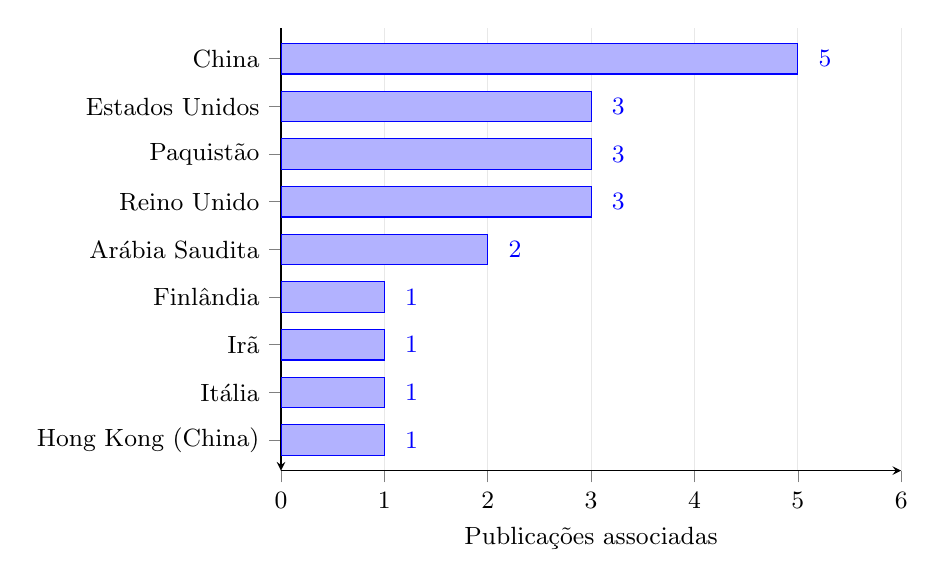
\begin{tikzpicture}
\begin{axis}[
  xbar, width=0.78\textwidth, height=7.2cm,
  xmin=0, xmax=6, xlabel={Publicações associadas},
  ytick={1,...,9},
  yticklabels={China,Estados Unidos,Paquistão,Reino Unido,Arábia Saudita,Finlândia,Irã,Itália,Hong Kong (China)},
  y dir=reverse, xtick={0,1,2,3,4,5,6},
  axis lines=left, tick align=outside,
  xmajorgrids=true, grid style={gray!18},
  tick label style={font=\small}, label style={font=\small},
  yticklabel style={font=\small},
  nodes near coords, nodes near coords style={font=\small\bfseries, xshift=4pt},
  bar width=11pt, enlarge y limits=0.08,
  every axis plot/.append style={fill=teal!65!blue, draw=teal!65!blue!80!black}
]
\addplot coordinates {(5,1) (3,2) (3,3) (3,4) (2,5) (1,6) (1,7) (1,8) (1,9)};
\end{axis}
\end{tikzpicture}
